\documentclass{IEEEtran}
\usepackage{graphicx}
\addcontentsline{toc}{chapter}{Bibliography}
\usepackage{amsmath}
\usepackage{amssymb}
\usepackage{algorithm}
\usepackage[noend]{algpseudocode}

\begin{document}


\title{Resource Allocation by Diversity}
\author{Yuri Lavinas}

\maketitle






\section{Introduction}

Multi-objective Optimization Problems (MOPs)~\cite{miettinen1999nonlinear} are problems composed by two or more functions which must be simultaneously optimized by the same set of parameters. This composition is characterized by a set of conflicting objective functions resulting in a set of optimal compromise solutions. 

These $m$ multiple objective functions must be optimized simultaneously:

\begin{align}\label{min_problem}
\text{minimize} f(x) = (f_1(x), ..., f_{m}(x)), \text{ with $x \in \mathbb{R}^{D}$},
\end{align}

where $m$ is the number of objective functions and $\mathbb{R}^m$ is the objective function space. $x \in \mathbb{R}^{D} = \{x_1, x_2, ..., x_D\}$ is a D-dimensional vector and it represents a candidate solution with ${D}$ variables, $f: \mathbb{R}^{D} \rightarrow \mathbb{R}^{m}$ is a vector of objective functions.% and $\Omega$ is the feasible decision space. $\Omega$ is defined as:

%\begin{align}
%\Omega =\{x \text{ in } \mathbb{R}^{n_v} | g_i(x) \leq 0 \text{ } \forall_i \text{ and } h_i(x) = 0 \text{ } \forall_j \},
%\end{align}
Objectives often conflict with each other therefore no point in $\Omega$ minimizes all the objectives at the same time. Consequently, the goal of MOP solvers is to find the best trade-off that balances the different objectives in an optimal way.

Given two feasible solutions vectors $u, v$ in $\Omega$, $u$  Pareto-dominates $v$, denoted by $f(u) \prec f(v)$, if and only if $f_k(u) \leq f_k(v), \forall_k \in \{1,..., m\}$ and $ f(u) \neq f(v)$. 

A solution $x \in \mathbb{R}^{D}$ is considered Pareto-Optimal if there exists no other solution $y \in \mathbb{R}^{D}$ such that $f(y) \succ f(x)$, i.e., if $x$ is non-dominated in the feasible decision space. A point is called non-dominated if no other point dominates it. That is, no single solution provides a better trade-off in all objectives.

The set of all Pareto-optimal solutions is known as the Pareto-Optimal Set (PS), while the image of this set is referred to as the Pareto-optimal Front (PF).\\

\begin{equation}
PS = \{x \in \Omega | \nexists y \in \Omega : f(y) \succ f(x^*)  \},
\end{equation}

\begin{equation}
PF = \{f(x) | x \in PS \}.
\end{equation}

Multi-objective evolutionary algorithms (MOEAs) are characterized by their ability to find good approximations the PF of a MOP in a single run~\cite{zhou2011multiobjective}.Over the last two decades, many different search techniques were proposed for improving the effectiveness of multi-objective algorithms. Among them, three are the major paradigms: Pareto domination-based approaches~\cite{deb2002fast},~\cite{zitzler2001spea2}, the indicator-based approaches~\cite{beume2007sms},~\cite{zitzler2004indicator}, and the decomposition-based approaches~\cite{li2009multiobjective},~\cite{zhang2007moea}. 


MOEA/D~\cite{zhang2007moea} represents a class of population-based meta-heuristics for solving Multi Objective Problems~\cite{trivedi2017survey}. In this search paradigm, the original multi-objective problem is decomposed into simpler, single-objective subproblems by means of scalarizations, see Figure~\ref{fig1}.
However, it may waste functions evaluations searching in directions that do not present Pareto-optimal solutions~\cite{bezerra2015comparing}. As in the example of Figure~\ref{fig2}, some vector represent "empty regions" of the PF.
\begin{figure}[h]
	\centering
	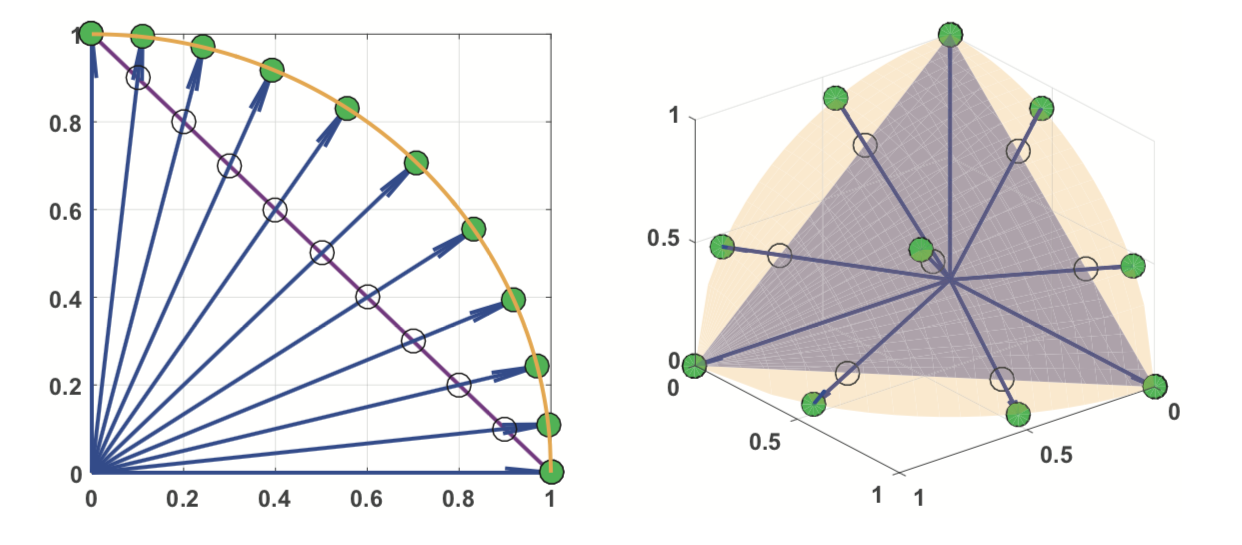
\includegraphics[width=0.55\textwidth]{img/decomp2.png}
	\caption{A decomposition strategy generates weight vectors that defines the subproblems. Figure from~\cite{chugh2017handling}.}
	\label{fig1}
\end{figure}

\begin{figure}[h]
	\centering
	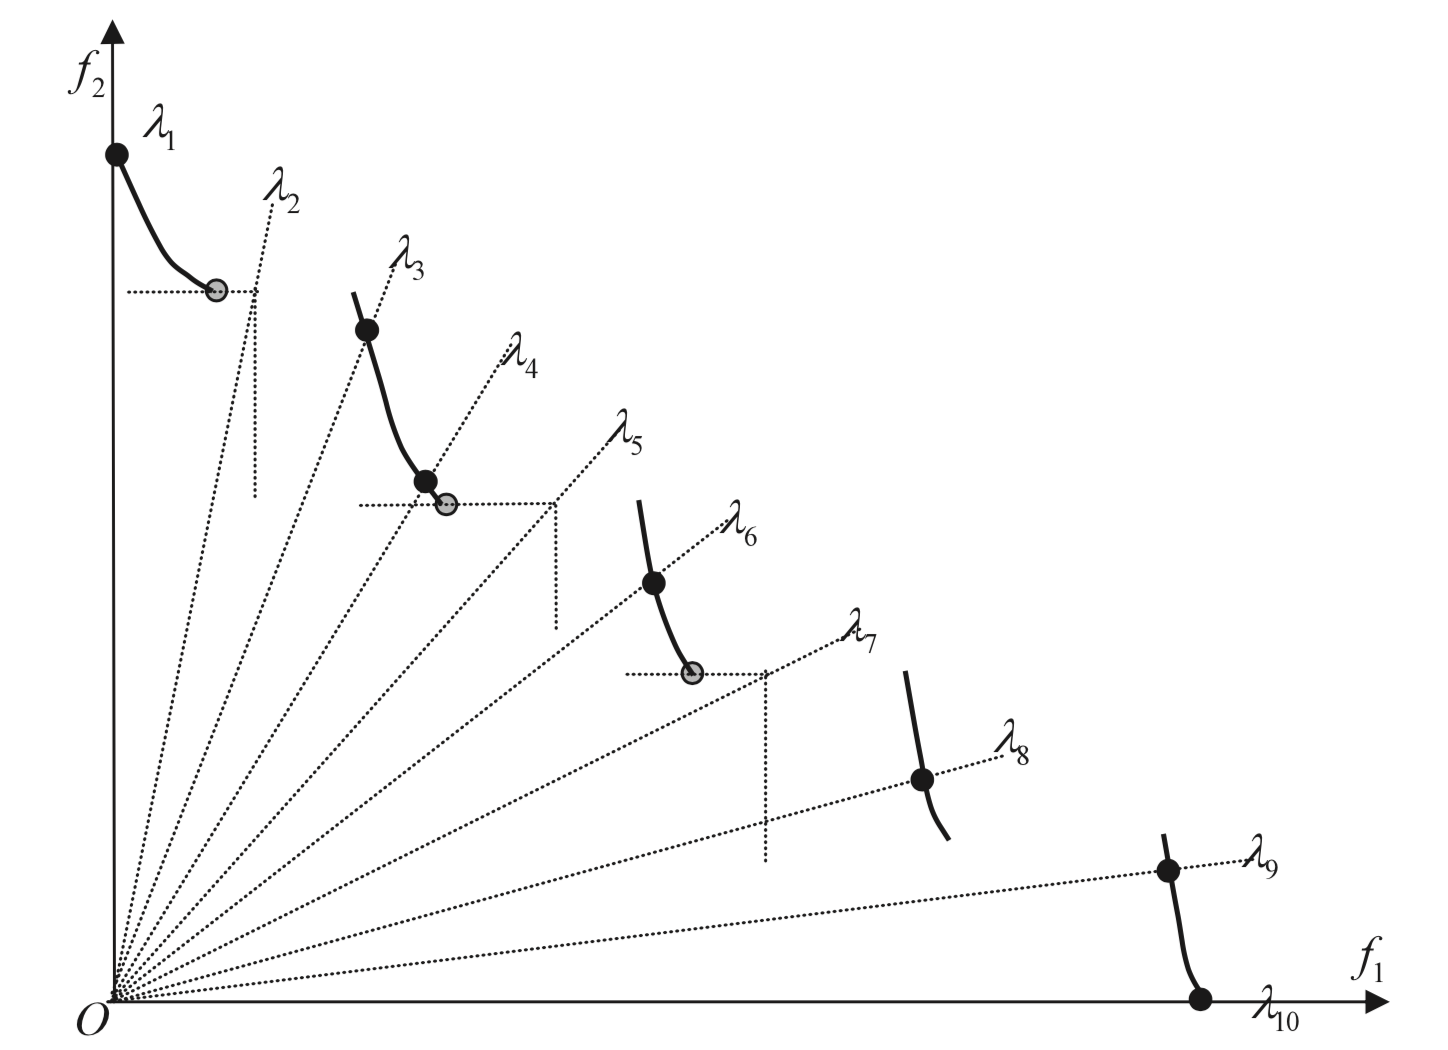
\includegraphics[width=0.43\textwidth]{img/harder_problems}
	\caption{Distribution of optimal solutions of subproblems with uniform weight vectors on ZDT3. Figure from~\cite{li2015use}.}
	\label{fig2}
\end{figure}


\begin{figure}[h]
	\centering
	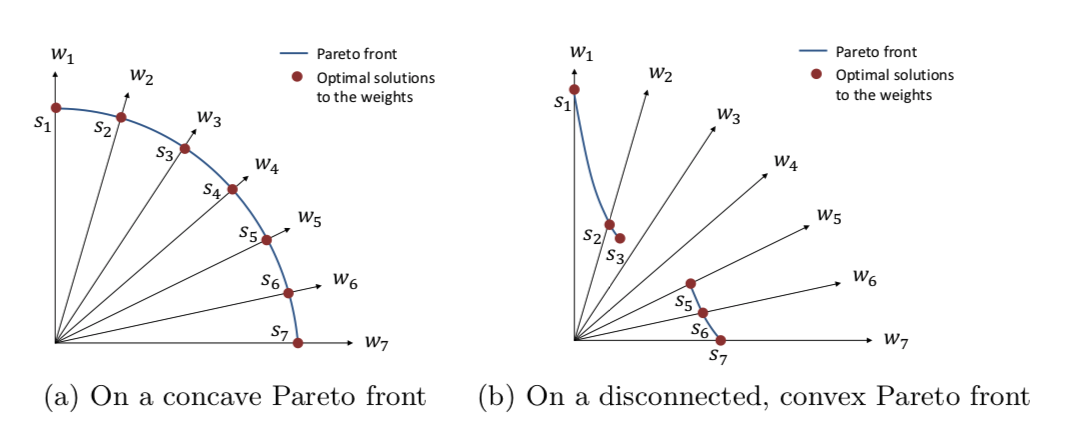
\includegraphics[width=0.53\textwidth]{img/harder_problems2}
	\caption{An example that uniformly distributed weights may lead to different distributions of optimal solutions. (a) Solutions $s_1$ to $s_7$ are the optimal solutions of weights $w_1$ to $w_7$, respectively. (b) Solutions $s_1$,$s_2$,$s_3$,$s_6$ and $s_7$ are the optimal solutions of $w_1$,$w_2$,$w_3$,$w_6$ and $w_7$, respectively, while solution $s_5$ is the optimal solution of $w_4$ and $w_5$.Figure from~\cite{li2017weights}}
	\label{fig3}
\end{figure}

In the original MOEA/D~\cite{zhang2007moea}, all the subproblems have the same amount of computational resource (number of iteractions). It has been observed, as one can expect that some parts of the theoretical Pareto Front PF, in an MOP can be more difficult to approximate than others, Figure~\ref{fig3},~\cite{zhang2009performance}~\cite{zhou2016all}~\cite{kang2018collaborative}.

%It represents a class of population-based meta-heuristics for solving MOPs. Many other algorithms exists as NSGA-2(3), MOEA/Ds, IBEA, SPEA2, DEMO.

This difficulties on approximating the PF may lead to a unbalanced exploration of the search space. One of the reasons is that, given to this dissimilar conditions, the number of iteractions needed will possibly not be the same. 

 To reduce this computational cost, the allocation of resources may be better distributed among different sub-problems according to their difficulties. One way to address this problem is to adjust the behavior of the algorithm in an on-line manner to suit the problem in question~\cite{hinterding1997adaptation},~\cite{de2007parameter},~\cite{meyer2007self},~\cite{zhang2009performance},~\cite{kramer2010evolutionary},~\cite{zhang2012survey}~\cite{cai2015external}. All algorithmic components can be tunned adaptively and often feedback information is needed for these adaptation strategies. 

Another way, is to allocate different amounts of resources to the subproblems based on some priority function. In a few recent works recently proposed, a utility function is being used to distribute the resources given priorities to subproblems that contribute more to the algorithm's search.  In the works of Zhang et al.~\cite{zhang2009performance} and Zhou et al.~\cite{zhou2016all} the a utility function was proposed aiming to prioritize solutions based on a historical convergence information during different generations. Another approach was implemented in~\cite{kang2018collaborative}, where the utility function was based on the presence of a solution from the main population on a secondary population.

The main contributions of this paper can be summarized as follows:

\begin{itemize}
	\item blablabla
	\item blebleble
	\item bliblibli
\end{itemize}

This work is divided in sections and subsections according to this and that.

\section{Related Works}

\subsection{Utility functions}


Utility functions are one way of defining priorities~\cite{chankong1983multiobjective},\cite{hansson2005decision},  and may be used as one way of deciding computational resources distributions among subproblems by guiding the distribution over generations~\cite{cai2015external}. 


To the best of the authors knowledge most of the works related to utility functions and resource allocation are: MOEA/D-DRA~\cite{zhang2009performance}, MOEA/D-GRA~\cite{zhou2016all}, MOEA/D-CRA~\cite{kang2018collaborative}, MOEA/D-AMS~\cite{chiang2011moea}. In these work an utility function, $u$, is used but without a clear justification. 

Zhou and Zhang~\cite{zhou2016all} claim that MOEA/D-GRA may be seen as an extension of MOEA/D-DRA and MOEA/D-AMS. The reason is that in MOEA/D-DRA and in MOEA/D-AMS some unsolved subproblems  are chosen for evolution in each generation according to their utility functions. For both MOEA/D-DRA and MOEA/D-GRA, the utility function, $u = \{u_1, u_2, ..., u_N\}$ for every subproblem $i=1,...,N$, is as defined in the next equation.
\begin{equation}\label{utility}
	u_i = \dfrac{\text{old fun val}-\text{new fun val}}{\text{old fun val}},
\end{equation}


supported by the idea that if a subproblem has been improved over the last $\Delta T$ generations (\textit{old function value}), it should have a high probability to be improved over the next few generations. While MOEA/D-CRA is based on a MOEA/D variation with two populations. Their utility function is based on if of an individual from population $A$ is selected to compose the population $B$.

My proposal is to integrate utility function with a diversity metric based on a geometrical interpretation of convergence and diversity to MOEA/D-GRA, given its straightforward implementation and integration with other MOEA/D variants.

%Why use MOEA/D-GRA?
%
%\begin{itemize}
%	\item It was easier to understand the proposal and in general had better results that MOEA/D-DRA~\cite{zhou2016all}.
%	\item Based on a more common and simpler MOEA/D than the MOEA/D-M2M.
%	\begin{itemize}
%		\item It is trivial to alter the variation of MOEA/D used as base.
%	\end{itemize}
%\end{itemize}

\subsection{Diversity Metric}

Here, I use MRDL as a way to assess the diversity of solutions in an on-line manner and use a utility function based on the output of this metric to guide resource allocation at each generation. 

The hyper-volume indicator (HV) or the Inverted Generational Distance (IGD)  could be used as the diversity metric. However both of them include information about convergence and diversity in a single metric.

There are mainly two groups metrics, the off-line ones, that calculate the diversity after the execution of the algorithm, and the on-line, that calculate the diversity during the execution of the algorithm. 

\paragraph{Off-line metrics} Chi-square-like deviation~\cite{deb1989genetic}, Spacing method~\cite{scott1995fault}, Uniformly distribution index~\cite{tan2002evolutionary}, Entropy approach~\cite{farhang2002diversity}, Grid diversity metric~\cite{deb2002running}, sparsity measure~\cite{deb2003fast}, and many others. 

They need knowledge of the PF or the ideal vector.

\paragraph{On-line metrics}sigma method~\cite{mostaghim2003strategies}  (PF lies in the positive objective space), 
entropy of the solutions by using Parzen window density estimation-\cite{tan2008evolutionary} (sensitive to kernel width), maximum relative diversity loss~\cite{gee2015online} (expensive $O(N^2)$, with $N$ being the size of the parent population).

In this work the maximum relative diversity loss was chosen to an online diversity assessment to measure the diversity loss caused by any individual in the population, for future works other metrics could be introduced.



\section{Proposed Method}

MOEA/D with on-line Resource Allocation by Diversity metric, MOEA/D-RAD, is a variant of MOEA/D that used a diversity metric as a way to select values for the utility function. Besides having a utility function based on a diversity metric, the algorithm is the same as MOEA/D-DE~\cite{li2009multiobjective}.

\begin{algorithm}[h]
	\caption{MOEA/D-RAD}\label{alg1}
	\begin{algorithmic}[1]

	\State Initialize the weight vectors $\lambda_i$, the neighborhood $B_i$, the utility value $u_i$ every subproblem $i=1,...,N$.
		
		\While{\textit{Termination criteria}}
		\For {1 to N}
			\If{$\textit{rand()} < u_i$}\Comment{From MOEA/D-GRA}
				\State Generate a offspring $y$ for subproblem $i$.
				\State Update the population by $y$.
			\EndIf
	\EndFor
	\State Update \textit{\textbf{u}} using a diversity metric.\Comment{Introduced here.}
		\EndWhile
	\end{algorithmic}
\end{algorithm}


The algorithm~\ref{alg1} describe MOEA/D-RAD. Except from line 4 and 7, the whole procedure in algorithm~\ref{alg1} is as in MOEA/D-DE. Likewise, all reproduction procedures are the same as in MOEA/D-DE~\cite{li2009multiobjective}. We initialize the value of the vector $u=0.5$ as in~\cite{zhou2016all}. A sensitivity analyzes need to be performed for deciding suitable values for $u$.

\section{Maximum Relative Diversity Loss (MRDL)} 

\begin{figure}[!t]
	\centering
	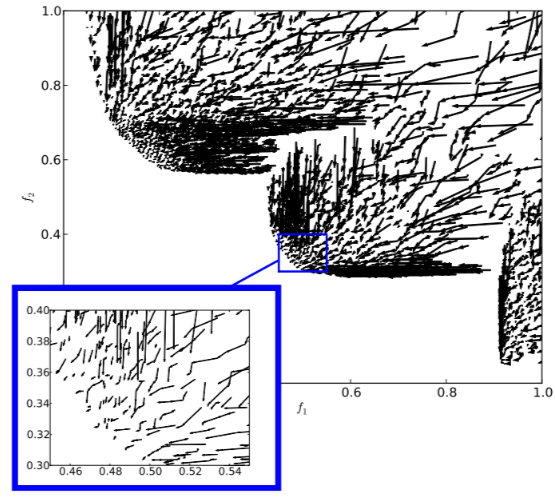
\includegraphics[width=0.47\textwidth]{img/conv_dir}
	\caption{Estimated convergence directions over 500 generations in CEC-09 UF1 benchmark test problem.Figure from~\cite{gee2015online}}
	\label{fig4}
\end{figure}

Maximum relative diversity loss (MRDL) is used to estimate the diversity loss of a solution to the whole population~\cite{gee2015online}.

 Some properties and implications of the MRDL:
\begin{itemize}
	\item If a new offspring generated is identical to any offspring solution in the convergence archive, $\Gamma^{p \rightarrow c}$  will be infinite.
	\item High values of $\Gamma^{p \rightarrow c}$ indicates the existence of similar offspring solution in the convergence archive or the offspring solution is close to the line of estimated convergence direction. 
\end{itemize}

The idea of the MRDL is to use the space movement (convergence directions) of a solution on the objective space towards the PF, as can be seen in Figure~\ref{fig4}, to calculate the diversity of the population. The further a objective vector of a solution is from the convergence direction, more it contributes for the diversity of the approximated PF.

%This is done since the convergence direction is perpendicular to the diverse direction. Here we use the definition of convergence as solutions approaching to the POF in the objective space for the first, while for diversity as the spreading and distribution of solutions along the PF~\cite{gee2015online}.


The main idea of calculating Maximum Relative Diversity Loss MRDL, $\Gamma^{p \rightarrow c}$, is to use it as a utility function as follows.

\begin{equation}
u_i = \Gamma^{p \rightarrow c}_i \text{ , with  $i=1,...,N$.}
\end{equation}

\begin{equation}
u_i = (u_i - min(u_i)) / (max(u_i) - min(u_i))
\end{equation}

\paragraph{MRDL} To calculate the MRDL, we need to compute $k$ convergence directions at every generation and then estimate the Relative Diversity Loss (RDL) for each of these $k$ convergence directions. Therefore, to estimate the diversity loss of a solution to the whole population by:
 
For every incumbent solution related to a subproblem $i$, from the whole population.

\begin{equation}
\Gamma_{i}^{p \rightarrow c} = \underset{i=1,...,k}{\max} \Gamma_{d.conv_{y}}^{p \rightarrow c}
\end{equation}


\paragraph{RDL.} RDL is a diversity measurement quantity that indicates the amount of diversity loss of an individual solution between two consecutive generations. High values of RDL imply a reduction of the solution spread and this equation may indicated the amount of diversity loss.

This quantity is given by a division between the shortest distance of a parent and offspring to the line of convergence direction.

\begin{equation}
\label{rdl}
\Gamma_{d.conv_{y}}^{p \rightarrow c} = \dfrac{ ||p \prime - proj_{d.conv_{y}}p \prime|| }{||c \prime - proj_{d.conv_{y}}c \prime||}
\end{equation}

The numerator in~\ref{rdl} is the closest distance between the parent solution ($p$) to the convergence direction $(c_r - p_r)$. While, the denominator in~\ref{rdl} is the closest distance between the offspring solution ($c$) to the convergence direction $(c_r - p_r)$. %The projections of $p\prime$ and $c\prime$ objective vectors onto the convergence direction $d.conv_{y}$ are $proj_{d.conv_{y}}p \prime$ and $proj_{d.conv_{y}}c \prime$.

with $p\prime$ and $c\prime $ given by:

\begin{equation}
\begin{split}
p\prime = p - p_r\\
c\prime = c - c_s\\
\end{split}
\end{equation}
%verify this

with $p_r$ and $c_s$ being the parent and offspring objective vectors used to calculate the convergence direction in equation~\ref{1}. That is the index $s$ is equal to the index $j$ used to calculate $conv_{y}$. The same principle is valid for the index $h$.
 
The vector projection between two vectors $a$ and $b$ that I used is defined as follows.

\begin{equation}
proj_{d.conv_{y}}p \prime = \frac {{d.conv_{y}} \cdot {p \prime}} {|{p \prime}|^2}{{p \prime}} 
\end{equation}

While the norm of $p \prime - proj_{d.conv_{y}}p \prime$ is calculated as follows.


\begin{equation}
||p \prime - proj_{d.conv_{y}}p \prime|| = sqrt(crossprod(proj_{d.conv_{y}}p \prime))
\end{equation}

The norm of $c \prime - proj_{d.conv_{y}}c \prime$ is calculated similarly.



\paragraph{Estimating convergence direction given weak-dominance relationship.}To estimate the convergence direction, $d.conv_{y}$, we need to have a offspring, $c_j$, that dominates a parent. Select a parent, $p_h$, solution that is closest to this offspring in the objective space. 

For every weakly dominated parent, one convergence direction is calculated as in the next equation.
\begin{equation}
\label{1}
	d.conv_{y} = c_j - p_h
\end{equation}

The index $j$ (for indexing offsprings, $c_j$) is selected from the set $D_c$.

\begin{equation}
\label{D}
	D_c = \{d| \exists c_d \prec p_k, k \in {1,..., N}, d \in [1,..., |C|]\}
\end{equation}

$N$ is the parent population size, $|C|$ is the size of the offspring population $C$. In equation~\ref{D}, the offspring $c_d$ must weakly dominate at least one parent solution. 

As from Zitzler et al.~\cite{zitzler2003performance} study, weak dominance ($A \succeq B$) means that any solution in B is weakly dominated by a solution in A. However, this does not rule out equality, because $A \succeq A$ for all approximation sets $A \in \Omega$.

The index $h$ (for indexing parents, $p_h$) comes from the following two equations.
\begin{equation}
h = \underset{k \in D_p }{argmin} || p_k - c_j ||
\end{equation}

\begin{equation}
\label{D_p}
D_p = \{k| \exists c_j \prec p_k, k \in {1,..., N}\}
\end{equation}

$D_p$ in equation~\ref{D_p} denotes the index set of parent solutions which are weakly dominated by $c_j$ (the $j$ index comes from equation~\ref{D}).


%\paragraph{Estimating diversity direction given the convergence direction} Diversity direction is define in~\cite{gee2015online} as the direction which is perpendicular to the converge direction.






\bibliographystyle{IEEEtran}
\bibliography{sample}


\end{document}